\section{Optika v anizotropních multivrstvách}
\label{chap:optika-v-multivrstvach}

Cílem tohoto oddílu je představit teorii výpočtu transmisních a reflexních koeficientů (Jonesových matic průchodu a odrazu) obecných vrstevnatých struktur popsaných stupňovitým profilem tenzoru $\varepsilon$.
Vrstevnatou strukturou rozumíme takovou, která je homogenní v rovině kolmé na jednu osu -- tu zvolíme jako $z$ -- a rovina homogenity a všech rozhraní bude $xy$, viz obr. \ref{fig:vrstevnate-prostredi}.
Stupňovitým profilem zase rozumíme, že struktura je složená z konečného počtu vrstev, ve kterých je $\varepsilon$ konstantní.

\begin{figure}[htbp]
    \centering
    \includegraphics[scale=0.7]{./img/static/vrstevnate-silber.pdf}
    \caption{Vrstevnaté prostředí (multivrstva). Každá vrstva je homogenní v rovině $xy$ a má konstantní tenzor permitivity $\varepsilon$. \cite{silberQuadraticMagnetoopticKerr2019a}}
    \label{fig:vrstevnate-prostredi}
\end{figure}

Budeme řešit Maxwellovy rovnice \eqref{eqn:rot-E}, \eqref{eqn:rot-ZH}.
Vzhledem k homogenitě v rovině $xy$ lze psát
\begin{equation} 
\label{eqn:pricne-vlnove-vektory}
    \vec{E}(x,y,z)=\vec{E}(z) e^{i(k_xx+k_yy)} \,, \qquad \vec{H}(x,y,z)=\vec{H}(z) e^{i(k_xx+k_yy)} \,,
\end{equation}
kde příčné složky vlnového vektoru $k_x$ a $k_y$ jsou konstantní podél celé struktury i mimo ní.
Uvnitř každé vrstvy bude existovat i třetí složka $k_z$, bude se ale lišit v různých vrstvách.
Obecný postup je tedy řešit Maxwellovy rovnice zvlášť v každém prostředí, a řešení následně svázat pomocí okrajových podmínek.
 
Budeme následovat řešení Berremanovou metodou přenosových matic\cite{berremanOpticsStratifiedAnisotropic1972}.
S uvážením \eqref{eqn:pricne-vlnove-vektory} mají Maxwellovy rovnice maticový tvar
\begin{equation}
\label{eqn:Berreman-6x6}
    \begin{pmatrix}
        0 & +i\partial_z/k_0 & N_y & -1 & 0 & 0 \\
        -i\partial_z/k_0 & 0 & -N_x & 0 & -1 & 0 \\
        -N_y & N_x & 0 & 0 & 0 & -1 \\
        \varepsilon_{11} & \varepsilon_{12} & \varepsilon_{13} & 0 & +i\partial_z/k_0 & N_y \\
        \varepsilon_{21} & \varepsilon_{22} & \varepsilon_{23} & -i\partial_z/k_0 & 0 & -N_x \\
        \varepsilon_{31} & \varepsilon_{32} & \varepsilon_{33} & -N_y & N_x & 0
    \end{pmatrix}
    \begin{pmatrix}
        E_x \\ E_y \\ E_z \\ Z_0 H_x \\ Z_0 H_y \\ Z_0 H_z
    \end{pmatrix} = \begin{pmatrix} 0 \\ 0 \\ 0 \\ 0 \\ 0 \\ 0 \end{pmatrix} \,.
\end{equation}

Člen prvního řádu\footnote{Prvního řádu $\partial_z$.} nemá plnou hodnost; třetí a šestou rovnici lze přímo vyřešit a dosadit do ostatních.
Nejdříve ale zavedeme úsporný blokově maticový zápis
\begin{align}
\label{eqn:Berreman-blokove-znaceni}
    \rho = \begin{pmatrix}0 & 1 \\ -1 & 0\end{pmatrix}
    \,, \qquad E^\perp = \begin{pmatrix}E_x \\ E_y\end{pmatrix}
    \,, \, H^\perp = \rho \begin{pmatrix} H_x \\ H_y\end{pmatrix} = \begin{pmatrix} H_y \\ -H_x \end{pmatrix}
    \,, \\ \varepsilon^\perp=\begin{pmatrix}\varepsilon_{11} & \varepsilon_{12} \\ \varepsilon_{21} & \varepsilon_{22}\end{pmatrix}
    \,, \, \varepsilon^\vert=\begin{pmatrix} \varepsilon_{13} \\ \varepsilon_{23} \end{pmatrix}
    \,, \, \varepsilon^-=\begin{pmatrix} \varepsilon_{31} & \varepsilon_{32} \end{pmatrix}
    \,, \qquad N = \begin{pmatrix} N_x \\ N_y \end{pmatrix}
    \,.
\end{align}

Třetí a šestá rovnice mají tvar
\begin{equation}
    N^T \rho E^\perp + Z_0 H_z =0 \,, \qquad \varepsilon^- E^\perp + N^T H^\perp + \varepsilon_{33} E_z=0 \,,
\end{equation}
vyřešením, dosazením do \eqref{eqn:Berreman-6x6} a úpravou dostáváme
\begin{equation} 
\label{eqn:Berreman-master}
    \partial_z \vec{G}
    = i k_0 \Delta \vec{G}
    \equiv i k_0 \begin{pmatrix}
        -\frac{N\varepsilon^-}{\varepsilon_{33}} & 1-NN^T \\ \varepsilon^\perp - \frac{\varepsilon^\vert\varepsilon^-}{\varepsilon_{33}} - \rho NN^T \rho & - \frac{\varepsilon^\vert N^T}{\varepsilon_{33}}
    \end{pmatrix}
    \vec{G} \,.
\end{equation}
pro vektor příčných polí $\vec{G} = (E_x, E_y, H_y, -H_x)^T$ a označili jsme Berremanovu matici $\Delta$.
Složky $\vec{G}$ jsou právě ty, jejichž spojitost na rozhraní diktují okrajové podmínky, takže není třeba se jimi zabývat zvlášť; stačí řešit rovnici \eqref{eqn:Berreman-master}.
Uvnitř každé vrstvy (v oblasti s konstantním $\varepsilon$ a tedy maticí $\Delta$) je řešením maticová exponenciála
\begin{equation}
\label{eqn:Berreman-exponenciala}
    \vec{G}(z_2) = e^{ik_0\Delta(z_2-z_1)} \vec{G}(z_1) \,,
\end{equation}
která lze spočíst diagonalizací\footnote{Obecně vzato nemusí být diagonalizovatelná, dovoluje však maximálně dvounásobnou degeneraci (dva módy postupné $+z$ a dva $-z$), takže v nejpatologičtějším případě má Jordanův tvar dvou $2\times2$ bloků.} obecně nehermitovské $4\times 4$ matice $\Delta$.
Matice má 4 komplexní vlastní čísla odpovídající vlnovým vektorům příslušných vlastních módů, které lze rozdělit do dvou skupin:
dva módy šířící se ve směru $+z$ mají\footnote{Podle \eqref{eqn:Poynting} $S_z \propto E_xH_y-E_yH_x$.} $\Re\lbrace N_z \rbrace\geq0$, $\Im\lbrace N_z \rbrace\geq0$, $S_z\geq0$; zbylé dva se šíří ve směru $-z$ a platí pro ně opačné nerovnice.

Velmi důležitým rozdílem Berremanova přístupu oproti Yehově maticové algebře je,
že zatímco v Yehově metodě je diagonalizace a hledání vlastních módů nedílnou součástí již definice základních pojmů formalismu (tzv. dynamické a propagační matice),
v Berremanově metodě se uplatňuje pouze jako pomocný výpočet jinak již dobře definované maticové exponenciály \eqref{eqn:Berreman-exponenciala}.
Diagonalizace a hledání vlastních módů jsou vysoce nelineární operace, jsou singulární v okolí degenerací (limita izotropního $\varepsilon$, či směr paprsku shodný s optickou osou) a někdy v nich dokonce selhávají\cite{xuOpticalDegeneraciesAnisotropic2000,wuSingularitiesMatrixFormalisms2018,garibelloSingularityYehTransfer2020,bertrandGeneralAnalyticalTreatment2001}.

Tento rozdíl je zásadní v magneto-optice, kde nás často zajímají právě drobné odchylky od izotropní $\varepsilon$, a výsledky jsou vyjádřeny do prvního řádu v těchto odchylkách.
V Yehově formalismu je obtížné počítat derivace podle složek $\varepsilon$; v \eqref{eqn:Berreman-exponenciala} je to však jednoduché\cite{bertrandGeneralAnalyticalTreatment2001}.
Z uvedených důvodů v této práci používáme Berremanův formalismus, přestože magneto-optice z velké části dominuje Yehův.

Poruchová teorie v Berremanově formalismu je rozvedena v dodatku \ref{app:berreman}.

\subsubsection*{Odraz a průchod}

Předpokládejme, že se nám podařilo vyřešit \eqref{eqn:Berreman-master} a tedy najít matici $\mathfrak{M}$, která svazuje příčná pole na začátku $(L)$ a na konci $(R)$ multivrstvy, viz obr. \ref{fig:odraz-pruchod}
\begin{equation}
    \vec{G}_{(L)}=\mathfrak{M} \vec{G}_{(R)}
\end{equation}


Úloha průchodu a odrazu je typicky zadána tak, že na strukturu posvítíme svazkem s definovaným vlnovým vektorem a polarizací, takže jsou zadány amplitudy dvou módů na levé straně s $k_z < 0$ (svítíme zleva).
Druhou podmínku volíme, že nikdo jiný na strukturu nesvítí, takže amplitudy všech zbylých módů, které přinášejí energii směrem ke struktuře, jsou nulové; to jsou dva módy na pravé straně s $k_z > 0$.
Na každé straně nám tedy zbývají dva módy, jejichž amplitudy zvýbá určit.
Vstupní a výstupní prostředí je nutné v tomto kontextu definovat jako to první, u kterého již nelze zpětné odrazy považovat za koherentní s dopadajícím svazkem (např. kvůli prostorovému oddělení).
Např. pro odraz od vzorku na tlustém substrátu je nutné uvažovat jako výstupní prostředí substrát.

Na obou stranách si zvolíme pro $-z$ i $+z$ šířící se módy bázi lineárních polarizací, kterými definujeme Jonesovi vektory pro příslušné svazky (pro ilustraci viz obr. \ref{fig:odraz-pruchod})
\begin{equation}
    \vec{G}_{(L)}=\mathfrak{D}_{(L)} \begin{pmatrix} \J^-_{(L)} \\ \J^+_{(L)} \end{pmatrix} \,, \qquad
    \vec{G}_{(R)}=\mathfrak{D}_{(R)} \begin{pmatrix} \J^-_{(R)} \\ \J^+_{(R)} \end{pmatrix} \,,
\end{equation}
kde $\mathfrak{D}$ diagonalizuje $\Delta$ ve smyslu, že $\mathfrak{D}^{-1}\Delta \mathfrak{D}$ je diagonální.
V Yehově formalismu se nazývají dynamické matice a obsahují ve sloupcích příčná pole jednotlivých módů.
V případě degenerace není $\mathfrak{D}$ jednoznačné -- volbou $\mathfrak{D}$ volíme bázi Jonesových vektorů.

\begin{figure}
    \centering
    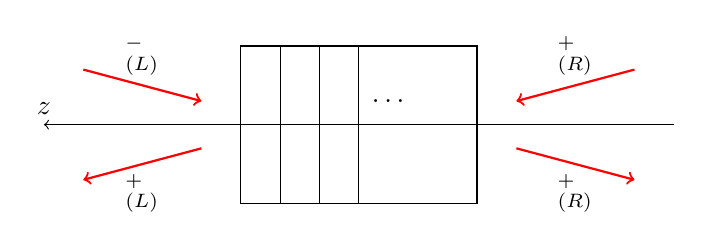
\begin{tikzpicture}[lase/.style={thick,color=red}]
    \draw[->] (4,0) -- (-4,0) node[anchor=south] {$z$};
    \draw (-1.5,-1) -- (1.5,-1) -- (1.5,1) -- (-1.5,1) -- cycle;
    \draw (-1,-1)--(-1,1) (-0.5,-1)--(-0.5,1) (0,1)--(0,-1);
    \path (0.4,0.3) node {\ldots};

    \draw[->,lase] (-3.5,0.7) -- node[color=black,anchor=south] {$\J^-_{(L)}$} (-2,0.3);
    \draw[<-,lase] (-3.5,-0.7) -- node[color=black,anchor=north] {$\J^+_{(L)}$} (-2,-0.3);
    
    \draw[->,lase] (3.5,0.7) -- node[color=black,anchor=south] {$\J^+_{(R)}$} (2,0.3);
    \draw[<-,lase] (3.5,-0.7) -- node[color=black,anchor=north] {$\J^+_{(R)}$} (2,-0.3);
\end{tikzpicture}


    \caption{Průchod a odraz od vrstevnatého prostředí. $(L)$, resp. $(R)$, značí veličiny na levé, resp. pravé straně multivrstvy. Polarizační stav dvojice módů šířících se ve směru $+z$, resp. $-z$, jsou popsány Jonesovými vektory $\J^+$, resp. $\J^-$.}
    \label{fig:odraz-pruchod}
\end{figure}

Častá volba $\mathfrak{D}$ v izotropním prostředí je báze lineárního příčného (TE, s-polarizace) a podélného (TM, p-polarizace) módu.
Zde ji uvedeme tak, abychom si usnadnili práci s téměř kolmým dopadem, nese to však s sebou přechod do báze odraženého světla s opačnou točivostí.
Opačný přístup volí opačné znaménko odražené p-polarizace, čímž se zachová točivost (viz např. \cite{silberQuadraticMagnetoopticKerr2019a}).
Souřadnou soustavu volíme tak, aby rovina dopadu byla rovnoběžná s jednou ze souřadných os, zde zvolíme $yz$, takže $N_x=0$, $N_y=\sin \alpha$, kde $\alpha$ je úhel dopadu.
Jako bázi módů volíme lineární polarizace příčné $J_s$ a podélné $J_p$ k rovině dopadu, viz. obr. \ref{fig:odraz-pruchod}.
Pro prostředí s indexem lomu $n$ má dynamická matice v této situaci explicitně tvar
\begin{equation}
    \vec{G} = \begin{pmatrix} E_x \\ E_y \\ Z_0 H_y \\ -Z_0 H_x \end{pmatrix}
    =\begin{pmatrix}
        1 & 0 & 1 & 0 \\
        0 & \cos\alpha_t & 0 & \cos\alpha_t \\
        -\cos\alpha_t & 0 & \cos\alpha_t & 0 \\
        0 & -1 & 0 & 1
    \end{pmatrix}
    \begin{pmatrix}
        J^-_{s} \\ J^-_{p} \\ J^+_s \\ J^+_{p} 
    \end{pmatrix} \,,
\end{equation}
kde jsme označili $\cos \alpha_t = \sqrt{1-\sin^2 \alpha /n^2}$ úhel lomu.

Při řešení průchodu a odrazu tedy pokládáme $\J^+_{(R)}=0$ a snažíme se vyjádřit zbylé prošlé $\J^-_{(R)} \equiv \J^t$ a odražené $\J^+_{(L)} \equiv \J^r$ pomocí známého dopadajícího $\J^-_{(L)} \equiv \J^i$, což lze pomocí matic $\mathfrak{M}$ a $\mathfrak{D}$ jednoduše z
\begin{equation}
    \begin{pmatrix} \J^i \\ \J^r \end{pmatrix}
    =\mathfrak{D}_{(L)}^{-1} \mathfrak{M} \mathfrak{D}_{(R)} 
    \begin{pmatrix} \J^t \\ 0 \end{pmatrix} \,,
\end{equation}
což vede na Jonesovy transmisní a reflexní matice Fresnelových koeficientů v bázi s- a p-polarizací
\begin{equation}
    \begin{pmatrix} J^r_s \\ J^r_p \end{pmatrix}
        =\begin{pmatrix} r_{ss} & r_{sr} \\ r_{ps} & r_{pp} \end{pmatrix}
        \begin{pmatrix} J^i_s \\ J^i_p \end{pmatrix} 
        \,, \qquad \begin{pmatrix} J^t_s \\ J^t_p \end{pmatrix}
        =\begin{pmatrix} t_{ss} & t_{sp} \\ t_{ps} & t_{pp} \end{pmatrix}
        \begin{pmatrix} J^i_s \\ J^i_p \end{pmatrix} \,.
\end{equation}

Multivrstva složená pouze z izotropních vrstev nemíchá s- a p-polarizaci, mimodiagonální členy jsou nulové.
Pokud je jedna nebo více vrstev pouze slabě anizotropní, projeví se to malými nenulovými mimodiagonálními členy.
Při dopadu např. s-polarizace pak prošlé a odražené světlo nabyde malé amplitudy p-polarizace, v elipsometrických parametrech se to projeví stočením hlavní roviny polarizace $\Delta \beta$ a elipticitou $\chi$; podobně pro dopadající p-polarizaci. 
Oba jevy souhrnně popisuje tzv. komplexní parametr stočení\cite{silberQuadraticMagnetoopticKerr2019a}, v reflexi s naší konvencí
\begin{equation}
\label{eqn:komplexni-rotace}
    \Psi_s \equiv \Delta \beta_s + i \chi_s \approx \frac{r_{ps}}{r_{ss}} 
    \,, \qquad \Psi_p \equiv \Delta \beta_p + i \chi_p \approx -\frac{r_{sp}}{r_{pp}} \,.
\end{equation}
V průchodu jsou reflexní koeficienty nahrazeny transmisními.
Komplexní parametr stočení se používá při popisu magneto-optických Kerrových jevů.
